\documentclass[sigconf]{acmart}
\settopmatter{printacmref=false, printccs=false, printfolios=true}
\renewcommand\footnotetextcopyrightpermission[1]{}


\usepackage{booktabs} % For formal tables




\begin{document}
\title{CAD Assignment 1}


\author{Hugo Werck 72692}
\email{h.werck@campus.fct.unl.pt}

\author{Marc Lichtner 72690}
\email{m.lichtner@campus.fct.unl.pt}


\begin{abstract}
The purpose of our work is to try different implementations on CUDA of a sequential version of the K-Means algorithm.
\end{abstract}


\maketitle

\section{Introduction}

% Refer to \verb|acmart.pdf| \cite{veytsmanlatex} (\url{https://www.ctan.org/pkg/acmart}, \url{http://www.acm.org/publications/proceedings-template}) for additional examples and instructions.

\subsection{K-Means and Its Application}

K-Means clustering is a widely used unsupervised machine learning algorithm which allows us to classify our data into groups based on their similarity. This technique is commonly used as the algorithm learns pattern on unlabelled data (i.e the algorithm is not given any predefined categories or outcome). Therefore, it is a particularly suitable technique on machine learning problems in which we don't have access to labelled data beforehand.

According to the article "What is k-means clustering" from IBM: "This type of cluster analysis is commonly used in data science for market segmentation, document clustering, image segmentation and image compression."

\subsection{Why Is It Interesting to Parallelize It, Particularly on GPUs}

Parallel computing is especially valuable when working with large datasets that contain at least one CPU-intensive component which can be broken into smaller, independent subtasks. This is the case for K-Means:

As K-Means is used for machine learning problems, it is often applied to large amounts of data. Furthermore, the two major steps of the algorithm consist of assigning each data point to the nearest cluster center and recomputing the center of each centroid based on those assignments. Both of these steps are computationally expensive and naturally independent, as each point’s distance to centroids can be computed separately, and the partial sums for each centroid update can be computed in parallel and then aggregated. Finally, as K-Means involves performing the same calculations for each point relative to the centroids, it is well-suited for SIMD operations on GPUs.

\subsection{What Is the Paper About}

This paper presents the implementation of the K-Means algorithm on NVIDIA GPUs using CUDA. We begin by analyzing a sequential implementation, identifying hotspot sections suitable for parallelization, and then propose a CUDA-based program with optimizations. Finally, we evaluate the performance gains achieved by our GPU-accelerated version through a series of experiments.

\section{Parallelizing KMeans on GPUs}

\subsection{Presentation of the Kmeans algorithm}

The K-Means algorithm takes as an input a number of clusters K, a set of m points where each point is defined as a vector representing the position of the point and containing a value for each of the n dimensions.

The idea of the algorithm is to initialize the centroids randomly and then proceed to iteratively perform those two main steps until convergence:
\begin{enumerate}
  \item \textbf{Assignment step:} Iterate through every points and calculate for each of them the Euclidean distance to every centroid in order to assign the closest centroid to this point. \\
\item \textbf{Update step:} Iterate through every centroid and calculate the mean of every position of its related points. Update the new position of the centroid with this value.
\end{enumerate}

These steps continue until there is no significative change anymore.

\subsection{Finding the parallelization candidates: our methodology for finding and choosing the code to parallelize}

The methodology used in order to find the code to parallelize was decomposed in two main parts:

1) By our original knowledge about the K-Means algorithm and with what we describe earlier, we already had a vague idea of parallelization opportunities that could be interesting: the two main steps of the algorithm we described above. Therefore, the first part of our approach involved reviewing the code in order to get a good understanding of the implementation and particularly with the assignment and update steps.
During this review, we identified three key parts of kmeans() that could be worthy to parallelized:
\begin{itemize}
  \item Distance calculation: The part where euclideanDistance() is called for
every combination of points and centroids .
\item Centroid update: The part of the algorithm that computes the new position for the centroids.
\item Assignment of points to clusters: The part of the code responsible of finding the new closest cluster for each point
\end{itemize}

2) Secondly, we wanted to confirm our first intuition with a profiler. We used perf to profile the sequential version of the code. This emphasized how computationally expensive the euclideanDistance() function is, as 95\% of the CPU time is spent on this specific function.
However, it is crucial to note that it is not the function itself that is parallelizable but the part of kmeans() calling this function. Indeed, the function itself only computes the distance for a single point and a single centroid whereas in kmeans(), it is called for every couple of points and centroids. Therefore, it is this nested loop that is more interesting to parallelize. This part of the code is obviously the most important part to optimize, as it represents a huge part of the CPU computation time.
To get a better understanding of the CPU time spent on updating the centroids, we put the code in an external function. The profiler showed that it represented 0.09\% however we wanted to check if we could get improvements in the code even if it  doesn't represented a big amount of CPU time.

\begin{figure}[h!]
    \centering
    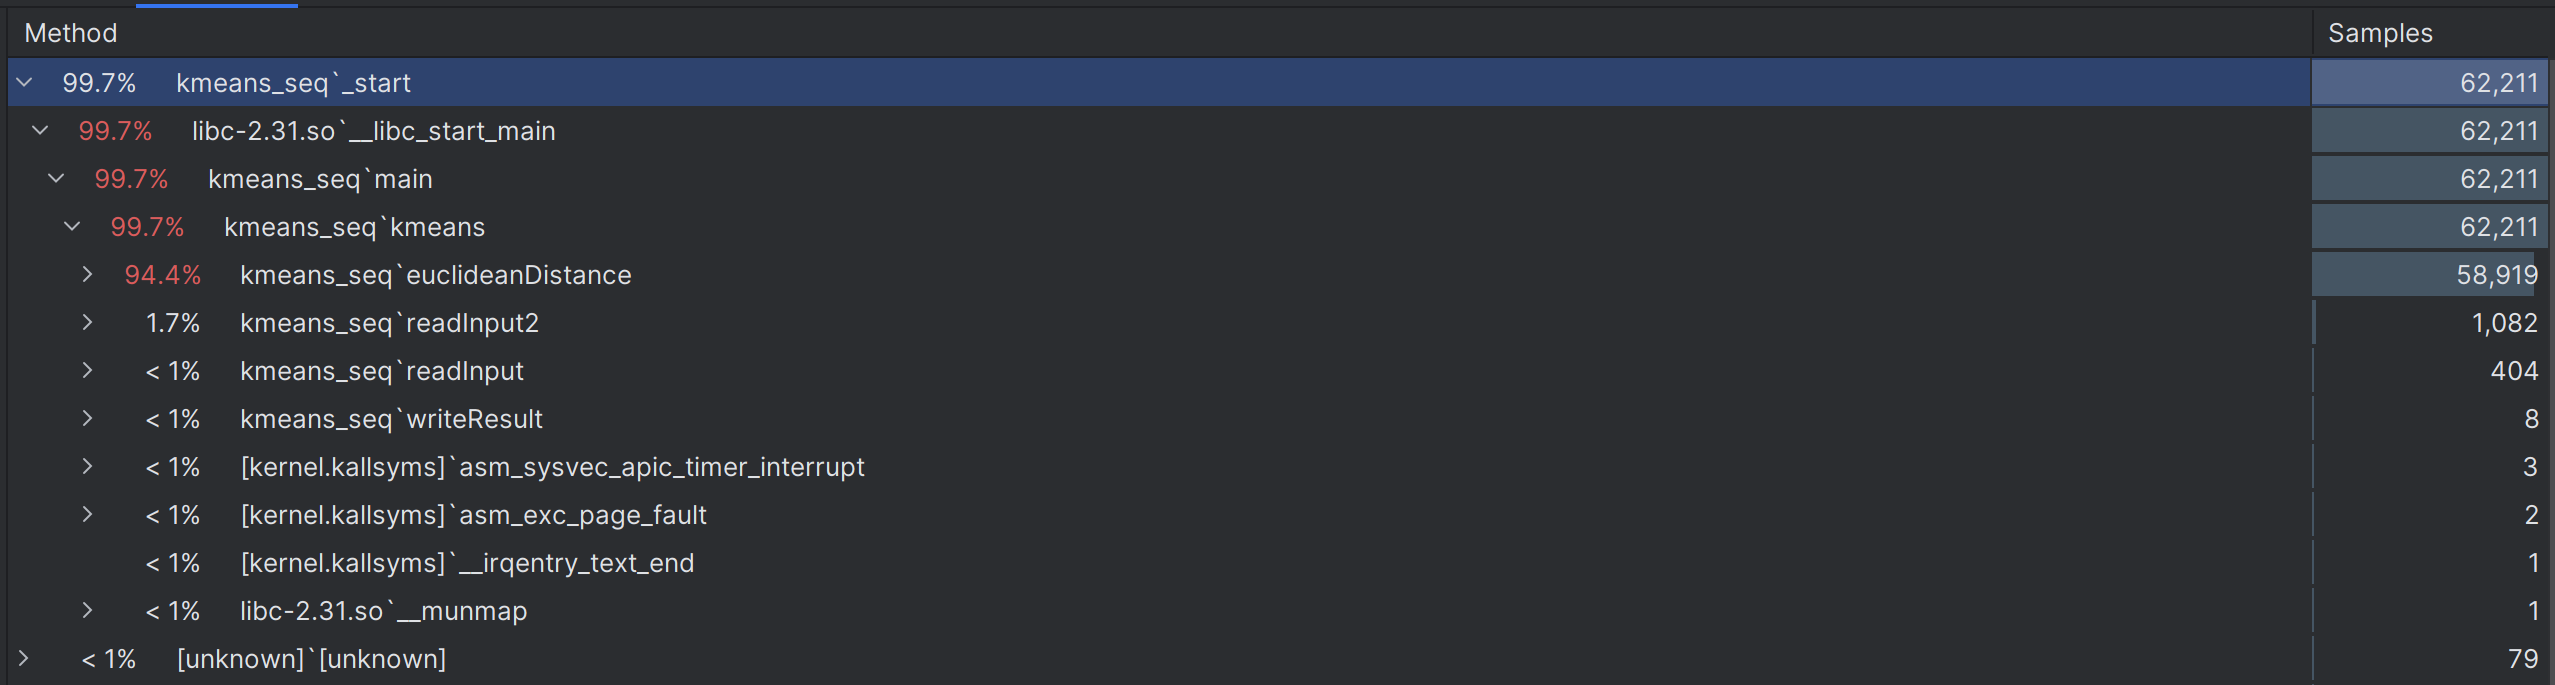
\includegraphics[width=\columnwidth]{initial_profiling.png}
    \caption{Initial profiling of the sequential program}
    \label{fig:initial_profiling}
\end{figure}

\subsection{Parallelization strategy for each candidate}

\subsubsection{Computation of the centroids position}
The parallelization strategy to optimize the calculation of the centroids position was done in two main steps.
First of all, we implemented a version in which each point corresponds to a thread. Each thread adds the value of the related point in the global memory. We knew that this version would not do such a difference due to contention on global memory but it allowed us to have a first working CUDA version of the algorithm.
From there, we made a new version of the algorithm in which we use shared memory to improve the performance. In this version, each block accumulates partial sums in shared memory. They are added to the global memory at the end of the kernel.
In this version, we split the shared memory space in two variables: sharedCentroidSums and sharedPointsPerClass. sharedCentroidSums contain for every centroid the sum of the coordinates of every related points. Therefore, for each centroid, there is d entry in the array where d is the number of dimensions.
sharedPointsPerClass contain for every centroid the number of points related to them. Therefore, the size of this array is the number of clusters.
With this in mind, we can compute the required size of shared memory we need and we can verify if it fits and we can specify the exact amount of shared memory when launching the kernel.
The amount of shared memory needed is given by: \emph{nbCluster*nbDimensions*sizeof(float) + nbCluster*sizeof(int)}.
Also the maximum size of shared memory for a block is 49152 bytes on the cluster.
We kept the two version of this function in order to use the version without shared memory in case the data would not fit in shared memory.
Indeed, after doing the calculations, we found that it would be exceeded. For example, we need at least 4096 clusters and 2 dimensions or 3072 clusters and 3 dimensions. This is unlikely because we won't need it in most case but it is not impossible as the K-Means algorithm is used in problem involving complex data or requiring very precise clustering.

\subsubsection{Computation of Euclidean Distance}
As mentioned before, the Euclidean distance calculations forms the most computationally intensive portion of the K-means algorithm. We implemented a CUDA kernel to parallelize this computation, where each thread calculates the distance from one point to one centroid. This approach allows us to process multiple point-centroid pairs in parallel. Thread organization was configured with a 2D block structure to optimize memory access patterns. We used a grid dimension that ensures all points and centroids are covered efficiently.

\subsubsection{'Full' version} We implemented all our optimizations in a single file: CUDA kernels for both Euclidean distance and centroid computations. For centroid calculations, we used shared memory to optimize performance, significantly reducing global memory accesses by locally accumulating centroid sums within each thread block before globally aggregating them. Our implementation dynamically checks if sufficient shared memory is available on the GPU and falls back to a non-shared memory version if necessary.

\subsection{Our overall optimizations}
Our overall optimization strategy focused on memory access along with efficiently using all of the GPU resources. We did implement each of the following improvements here. They supplement the kernel-specific optimizations described earlier on.
\begin{itemize}
    \item Our implementation minimized host-device transfers for it kept intermediate results in device memory throughout the algorithm's execution, also it transferred data between CPU and GPU only when necessary.
    \item Thread block dimensions were optimized with 16×16 threads for distance calculations and 256 threads for point-based operations, improving GPU efficiency across different calculation types.
    \item At runtime, when checking GPU capabilities, we implemented adaptive usage of shared memory. Our code does fall back in a dynamic way if the memory that is required exceeds shared memory which is available per block. Then the non-shared memory becomes implemented.
    \item Before global aggregation to reduce global memory traffic, shared memory for centroids collected centroid sums locally inside each thread block.
    \item We counted classification changes directly on the GPU using atomic operations, avoiding unnecessary data transfers to the CPU for convergence checks.
    \item The parallel kernel we built locates the closest centroid because it handles all data points at once instead of one by one, increasing speed on huge datasets.
\end{itemize}


\section{Experimental results}

\subsection{Questions we you want to answer with our experiments}

\begin{enumerate} 
    \item How much time could we gain using CUDA compared to CPU on such a complex problem? 
    \item What are the advantages and drawbacks of using CUDA to compute the K-Means? 
    \item How do our specific optimizations affect performance across different dataset characteristics?
    \item How does our implementation scale with increasing dataset size and varying numbers of clusters (K)? 
    \item Under what conditions is CUDA parallelization most beneficial?
    \item When is the usage of GPU computation not justified?
    \item Could we get improvements by parallelizing part of the code, even though this part is not computationally intensive? 
\end{enumerate}

\subsection{Our methodology}


To exhaustively evaluate our implementations, we designed a test suite with varying datasets and parameters:

\paragraph{Datasets:} 
\begin{itemize}
    \item \texttt{input2D.inp}: Small dataset with 2-dimensional points
    \item \texttt{input10D.inp}: Medium dataset with 10-dimensional points
    \item \texttt{input100D2.inp}: Large dataset with 100-dimensional points and 100,000 points
\end{itemize}

\paragraph{Implementations:} 
\begin{itemize}
    \item \textbf{Sequential}: Baseline CPU implementation
    \item \textbf{CUDA Centroids}: Only centroid calculations parallelized on GPU
    \item \textbf{CUDA Distances}: Only distance calculations parallelized on GPU
    \item \textbf{CUDA Full}: Both distance calculations and centroid updates parallelized on GPU
\end{itemize}

\paragraph{Parameter variations:} 
\begin{itemize}
    \item K (number of clusters): 10, 100, 500
    \item Iterations: 10, 100
    \item Change threshold: 0, 100
    \item Move threshold: 0.005, 0.4
\end{itemize}

\paragraph{Hardware/Software Setup:}
Marc worked remotely within CLion on the DI cluster (node bulbasaur). Hugo worked locally with WSL2 (Ubuntu) on Windows 11, using CMake and VSCode. The testing hardware included an AMD Ryzen 7745HX CPU and an Nvidia RTX 4070 GPU.


\subsection{Results}
\subsubsection{Performance across dataset dimensions}

For the 100-dimensional dataset with 100 clusters (K=100), we observed dramatic differences in performance:

\begin{table}[h]
\centering
\begin{tabular}{|l|r|r|}
\hline
\textbf{Implementation} & \textbf{Runtime (s)} & \textbf{Acceleration} \\
\hline
Sequential & 26.404945 & 1.00x \\
\hline
CUDA Centroids & 25.791713 & 1.02x \\
\hline
CUDA Distances & 1.189070 & 22.21x \\
\hline
CUDA Full & 0.772455 & 34.18x \\
\hline
\end{tabular}
\caption{Performance comparison for input100D2 with K=100}
\end{table}

However, for lower dimensional data (10D and 2D), the sequential implementation outperformed CUDA versions:

\begin{table}[h]
\centering
\begin{tabular}{|l|r|r|}
\hline
\textbf{Implementation} & \textbf{Runtime (s)} & \textbf{Acceleration} \\
\hline
Sequential & 0.025944 & 1.00x \\
\hline
CUDA Full & 0.314814 & 0.08x (12.5x slower) \\
\hline
\end{tabular}
\caption{Performance comparison for input10D with K=100}
\end{table}

\subsubsection{Scaling with number of clusters (K)}

We tested how performance scales with increasing K values on the 100-dimensional dataset:

\begin{table}[h]
\centering
\begin{tabular}{|r|r|r|r|}
\hline
\textbf{K value} & \textbf{Sequential (s)} & \textbf{CUDA Full (s)} & \textbf{Acceleration} \\
\hline
10 & 2.907249 & 0.736893 & 3.95x \\
\hline
100 & 26.404945 & 0.772455 & 34.18x \\
\hline
500 & 122.362469 & 0.897307 & 136.37x \\
\hline
\end{tabular}
\caption{Scaling performance with increasing K values}
\end{table}

\subsubsection{Acceleration per component}

Analysis of individual CUDA components shows that distance calculation parallelization provides the most significant performance boost:

\begin{table}[h]
\centering
\begin{tabular}{|r|r|r|r|r|}
\hline
\textbf{K} & \textbf{Centroids} & \textbf{Accel.} & \textbf{Distances} & \textbf{Accel.} \\
\hline
10 & 3.022040s & 0.96x & 0.933671s & 3.11x \\
\hline
100 & 25.791713s & 1.02x & 1.189070s & 22.21x \\
\hline
500 & 122.602122s & 1.00x & 2.074928s & 58.97x \\
\hline
\end{tabular}
\caption{Performance impact of individual CUDA components}
\end{table}

\subsection{Discussion}
In this section we will provide the answers we have found experimentally to the questions raised in Section 3.1:

\paragraph{Question 1.} 
For large-scale problems (high dimensions, many clusters), the performance improvement is impressive - up to 136x faster with K=500 and 100 dimensions. This acceleration becomes more significant as the problem size increases.

\paragraph{Question 2.}
\begin{itemize}
    \item \textbf{Advantages:} Huge performance gains for suitable problems, excellent scaling with problem size, enables processing of much larger datasets in reasonable time.
    \item \textbf{Drawbacks:} Implementation complexity (especially shared memory and thread synchronization), initialization overhead making it inefficient for small problems, and increased code complexity.
\end{itemize}

\paragraph{Question 3.}
Our experiments reveal that the distance calculation is the primary bottleneck in K-means. Parallelizing distance calculations gives a 22-59x acceleration depending on K, while parallelizing centroid updates alone provides minimal benefit (0.96-1.02x). 

\paragraph{Question 4.}
The sequential implementation scales badly with both dimensionality and K, showing quadratic growth in runtime. In contrast, our CUDA implementation scales excellently with increasing K values - runtime increases only slightly from K=10 (0.74s) to K=500 (0.90s) !

\paragraph{Question 5.}
CUDA provides the greatest benefits with:
\begin{itemize}
    \item High-dimensional data (100D vs 10D or 2D)
    \item Large numbers of clusters (K>=100)
    \item Large datasets (many points)
\end{itemize}

\paragraph{Question 6.}
For small problems (low dimensions, few clusters, or small datasets), the sequential implementation outperforms CUDA implementations. For example, with 2D data, the sequential implementation is 50x faster than CUDA. This demonstrates that GPU parallelization is not a universal solution but should be applied only on specific problems regarding their characteristics.

\paragraph{Question 7.}
After implementing a parallelized version of the computation of the new position for the centroids, the metrics showed that as this part of the code wasn't computationally intensive at first, it didn't made significant improvements.

\section{Conclusions} 

\subsection{What was achieved}
Our project allowed us to observe the potential of GPU computing for applications involving data clustering. By implementing K-means with CUDA, we achieved very surprising accelerations, on large, high-dimensional datasets, transforming hours of computation into seconds.

The most significant observation was the highly scaled impact of parallelizing the algorithm's various components. While parallelizing centroid updates provided only negligible benefits, parallelizing distance computation offered a very significant acceleration. This enormous contrast demonstrates the importance of identifying computational hotspots before parallelizing.

Our results allow us to establish that CUDA acceleration becomes exponentially more useful as the dimensionality and number of clusters increase, especially in conditions where traditional CPU implementations struggle the most. Interestingly, for small 2D datasets, our GPU implementation was actually way slower than the CPU, highlighting the significant cost of GPU initialization. That it is not suitable for every type of problem.

\subsection{Suggestions for improvements or future developments}

\paragraph{Hybrid execution:} Develop an implementation that dynamically switches between CPU and GPU depending of the problem characteristics to maximize performance.
\paragraph{Memory hierarchy optimization:} The distance calculation performance could be slightly improved by exploiting a bit more the GPU memory hierarchy, through a shared memory strategy.
\paragraph{Algorithmic innovation:} Explore different algorithmic approaches that might better exploit GPU's parallelism.
\paragraph{Importance of a proper profiling :} We spent time and effort implementing a parallelized version of the computation of the new centroid position, which was initially not a computationally intensive part of the sequential program. We obviously haven't seen improvements from this, which proves that even if this part was parallelizable and seemed like an interesting part during the code review, it wasn't worth, as it didn't lead to significant changes.
We now fully understand the value of proper profiling and that parallelizing hotspots is key to get performance improvements.

\section{bibliography}
\begin{itemize}
    \item \textbf{https://www.ibm.com/think/topics/k-means-clustering}
    This article has been useful and complemented quite well the information given in the subject about the K-Means algorithm.
    The relevant information we kept from this article is about the use cases of this algorithm:
    "This type of cluster analysis is commonly used in data science for market segmentation, document clustering, image segmentation and image compression. The k-means algorithm is a widely used method in cluster analysis because it is efficient, effective and simple."
    We used this part in the introduction in the section: K-Means and Its Application.
    \item \textbf{https://docs.nvidia.com/cuda/cuda-c-programming-guide/}
    We had to use CUDA official documentation for specific code questions, such as using the atomicAdd() function.
\end{itemize}

\section{acknowledgments}

For this project, we haven't really discussed a lot with other groups and focused on working in pair. 

\section{individual contributions}
We tried to distribute the work as equally as possible and we wanted to be sure that each of us were evolved in every step of the project.

However, some specialization naturally emerged over the course of the work. Marc primarily managed the code review and profiling whereas Hugo conducted most of the experiments on the results.

In terms of code, Hugo implemented the kernel for the euclidean distance and the kernel that computes the closest centroid for each point whereas Marc implemented both version of the kernel to compute the new position for the centroids. We both made the correspond change needed in the main function kmeans() to implement those kernels.

Hugo maintained the test script code and made the corresponding CMake modifications (a few CMakeLists.txt files) to allow the project to work according to our implementations.

The report was primarily written by Marc while Hugo authored section 3 and 4 and contributed to reviewing and refining the overall content as needed.

We tried to keep the workload balanced by regularly reassessing and redistributing tasks whenever we felt the distribution was becoming uneven. Therefore, we would say that a distribution with 50\% each (+/- 5\%) seems fair.

\section{comments, critics, and suggestions}

\paragraph{Marc:} I found this course very valuable because we needed to have a good understanding about what happens at the hardware level and how architectural constraints shape the way we code. Even though I felt overwhelmed by some lectures like lecture 4 about performance optimizations, the course sparked a good interest and I'm looking forward to revisiting the material at my own pace during summer.


\bibliographystyle{acm}

\end{document}